\documentclass[12pt, letterpaper]{article}

\setlength{\topmargin}{-1.75cm} \setlength{\textheight}{22.5cm}
\setlength{\oddsidemargin}{0.25cm}
\setlength{\evensidemargin}{0.25cm} \setlength{\textwidth}{16.2cm}

\usepackage{fdsymbol}
\usepackage{stmaryrd}
\usepackage{pifont}
\newcommand{\cmark}{\ding{51}}
\newcommand{\xmark}{\ding{55}}
\usepackage[ruled,linesnumbered]{algorithm2e}
\usepackage{graphicx}
\usepackage[linguistics]{forest}
\usepackage{tikz} 
\usetikzlibrary{automata,positioning}
\usepackage{palatino, url, multicol}
\usepackage{pictex}
\def\color#1]#2{}
\usepackage{fancyhdr}
\pagestyle{fancy}

\newcommand{\hwnumber}{3}
\newcommand{\hwtitle}{Foundation. Languages. Automata.}
\newcommand{\duedate}{11:59pm Friday October 10}
\newcommand{\set}[1]{\{#1\}}
\newcommand{\pg}[1]{{\tt #1}}
\newtheorem{definition}{Definition}
\newcommand{\emptyclause}{\Box}
\newcommand{\keyword}[1]{{\bf #1}}

\date{}

\begin{document}

\title{{\bf Homework \hwnumber.} \hwtitle}
\maketitle

%% Software Verification and Validation was part of collaboration with Professor Namin (see software-vv repository).
\noindent Software Verification and Validation was undertaken in collaboration with Professor Namin. See the software-vv repository for related work.

\vspace{1em}

\fancyhf{}
\thispagestyle{fancy}
\chead{\courseTitle\ by Y Zhang, TTU,\courseDate}
\cfoot{\thepage}

\noindent {\bf Submit both PDF and LaTeX file of your solution to Canvas by \duedate.}

\begin{enumerate}

\item You must use LaTeX for your submission.

\item Write a pseudocode algorithm where the input is a regular expression $R$ and the output is the language represented by $R$. 

\textit{Hint: Study the definition of semantics of regular expressions around page 59 of Lecture 3. Your pseudocode algorithm can be based on problem decomposition/divide and conquer using the definition.}

\textit{LaTeX sample algorithm format:}

\begin{algorithm}[H]
\SetKwInOut{Input}{Input}
\SetKwInOut{Output}{output}
\SetKwInOut{SideEffect}{side effect}
\SetKwInOut{Plan}{plan}
\SetAlgoLined
\Indm
\Input{$A[1..n]$: the array of numbers to sort and $n$ is the number of elements in array $A$.}
\Output{N.A.}
\SideEffect{The numbers in array $A$ is ordered}
\Plan{}
\Indp
\While{While condition}{
    instructions\;
    \eIf{condition}{
        instructions1\;
        instructions2\;
    }{
        instructions3\;
    }
}
\caption{sort}
\end{algorithm}

\noindent\textbf{ANSWER:}

\begin{algorithm}[H]
\SetKwInOut{Input}{Input}
\SetKwInOut{Output}{Output}
\SetKwInOut{Plan}{Plan}
\SetAlgoLined
\Indm
\Input{A regular expression $R$ over alphabet $\Sigma$}
\Output{The language $\mathcal{L}(R) \subseteq \Sigma^\ast$}
\Plan{Divide-and-conquer on the syntax of $R$ using the semantics of regular expressions}
\Indp

\SetKwFunction{Lang}{Lang}
\SetKwFunction{Kleene}{KleeneClosure}
\SetKwProg{Fn}{Function}{:}{end}

\Fn{\Lang{$R$}}{
  \uIf{$R = \emptyset$}{\Return{$\emptyset$}}
  \uElseIf{$R = \varepsilon$}{\Return{$\{\varepsilon\}$}}
  \uElseIf{$R = a$ for some $a\in\Sigma$}{\Return{$\{a\}$}}
  \uElseIf{$R = (R_1 \cup R_2)$}{\Return{$\Lang(R_1)\ \cup\ \Lang(R_2)$}}
  \uElseIf{$R = (R_1 R_2)$}{\Return{$\{\, xy \mid x \in \Lang(R_1)\ \wedge\ y \in \Lang(R_2)\,\}$}}
  \uElseIf{$R = (R_1)^\ast$}{\Return{\Kleene{$\Lang(R_1)$}}}
  \Else{\Return{\Lang{($R'$)} where $R'$ is the subexpression inside outer parentheses}}
}

\Fn{\Kleene{$L$}}{
  \Return{$\bigcup_{i\ge 0} L^{i}$ where $L^0 \triangleq \{\varepsilon\}$ and $L^{i+1} \triangleq \{\, xy \mid x\in L^i,\, y\in L \,\}$}
}

\caption{Semantic evaluation $\mathcal{L}(R)$ of a regular expression $R$}
\end{algorithm}

\item Consider the following NFA diagram:

\begin{center}
\begin{tikzpicture}[shorten >=1pt,node distance=2cm,on grid,auto] 
    \node[state,initial] (q_0) at (1.25,2.0) {$q_0$}; 
    \node[state](q_1) at (0,0) {$q_1$};
    \node[state, accepting](q_2) at (2.5,0) {$q_2$};
    \path[->] 
    (q_0) edge node {a} (q_2)
    (q_0) edge [above] node {a} (q_1)
    (q_1) edge [below] node {b} (q_2);
\end{tikzpicture}
\end{center}

Write a tuple representation of this automaton (using the notation from our definition of NFA).

\noindent\textbf{ANSWER:}

Let $N=(\Sigma,K,s,F,\Delta)$ be the NFA, where
\[
\Sigma=\{a,b\},\quad
K=\{q_0,q_1,q_2\},\quad
s=q_0,\quad
F=\{q_2\}.
\]
The transition function $\Delta:K\times\Sigma\to \mathcal{P}(K)$ is
\[
\begin{aligned}
&\Delta(q_0,a)=\{q_1,q_2\},\ \ \Delta(q_0,b)=\emptyset,\\
&\Delta(q_1,a)=\emptyset,\ \ \ \ \ \ \ \ \ \Delta(q_1,b)=\{q_2\},\\
&\Delta(q_2,a)=\emptyset,\ \ \ \ \ \ \ \ \ \Delta(q_2,b)=\emptyset.
\end{aligned}
\]

\item The \textbf{language} accepted by an NFA $N$ is the set of all strings accepted by the NFA. Write the definition of this concept using set builder notation.

\noindent\textbf{ANSWER:}

Let $N=(\Sigma,K,s,F,\Delta)$ and let $\vdash_N^\ast$ be the reflexive-transitive closure of one-step moves. Then
\[
L(N)\ \triangleq\ \{\, w \in \Sigma^\ast \mid \exists\, q_f \in F \text{ such that } (s,w)\ \vdash_N^\ast\ (q_f,\varepsilon)\,\}.
\]
Equivalently, letting $\Delta^\ast$ be the extended transition function,
\[
L(N)\ =\ \{\, w\in\Sigma^\ast \mid \Delta^\ast(\{s\},w)\ \cap\ F \neq \emptyset \,\}.
\]

\item Given the automaton diagram below and the string $0010$, draw the computation tree for processing $0010$ on this automaton.

\begin{center}
\begin{tikzpicture}[shorten >=1pt,node distance=2cm,on grid,auto] 
    \node[state,initial] (q_0) {$q_0$}; 
    \node[state](q_1) [right=of q_0] {$q_1$};
    \node[state, accepting](q_2) [right=of q_1] {$q_2$};
    \path[->] 
    (q_0) edge [loop above] node {$0,1$} ()
    (q_0) edge node {$0$} (q_1)
    (q_1) edge node {$1$} (q_2);
\end{tikzpicture}
\end{center}

\textit{LaTeX sample tree format (content is unrelated to the answer):}

\begin{center}
\begin{forest}
    [$q_0$, 
    [$q_1$, edge label={node[midway,left]{a}} 
    [$q_2$, edge label={node[midway,left]{b}}
    [\cmark, edge = dotted]
    ]
    ]
    [$q_2$, edge label={node[midway,right]{a}}
    [\xmark, edge = dotted]
    ]
    ]
\end{forest}
\end{center}

\noindent\textbf{ANSWER:}

\begin{center}
\begin{forest}
  for tree={grow'=0, child anchor=west, anchor=west, parent anchor=south, edge path={\noexpand\path [draw, ->] (!u.south) +(0,-2pt) -| (.child anchor)\forestOuline;}, l sep+=8pt}
  [$q_0$ on $0010$
    [$q_0$ on $010$, edge label={node[midway,left]{$0$}}
      [$q_0$ on $10$, edge label={node[midway,left]{$0$}}
        [$q_0$ on $0$, edge label={node[midway,left]{$1$}}
          [$q_0$ on $\varepsilon$, edge label={node[midway,left]{$0$}} [\xmark, edge=dotted]]
          [$q_1$ on $\varepsilon$, edge label={node[midway,right]{$0$}} [\xmark, edge=dotted]]
        ]
      ]
      [$q_1$ on $10$, edge label={node[midway,right]{$0$}}
        [$q_2$ on $0$, edge label={node[midway,left]{$1$}}
          [\xmark, edge=dotted, label=right:{no $0$-move from $q_2$}]
        ]
      ]
    ]
    [$q_1$ on $010$, edge label={node[midway,right]{$0$}}
      [\xmark, edge=dotted, label=right:{no $0$-move from $q_1$}]
    ]
  ]
\end{forest}
\end{center}

(All leaves reject on $0010$, so the string is not accepted.)

\item Consider these definitions:

A configuration $(q, w)$ \textbf{yields in one step} configuration $(q', w')$, denoted by $(q, w) \vdash_M (q', w')$, if $w = a w'$ and $\delta(q, a) = q'$. 

A configuration $(q_1, w_1)$ \textbf{yields} configuration $(q_2, w_2)$, denoted by $(q_1, w_1) \vdash_M^* (q_2, w_2)$, if there is a sequence of configurations, starting with $(q_1, w_1)$ and ending with $(q_2, w_2)$, each of which is yielded in one step from its previous configuration.

Answer the following: What concepts are being defined? What concepts are used in these definitions? What logical symbols appear? What are the important variables? What is the tree structure of the definition statement for \textit{yields}?

\noindent\textbf{ANSWER:}

They define (i) the \emph{one-step move} relation $\vdash_M$ and (ii) its \emph{reflexive-transitive closure} $\vdash_M^\ast$ (``yields'') for a machine $M$. Concepts used: configurations $(q,w)$, the DFA transition function $\delta$, decomposition of an input string $w = a w'$, and finite sequences of configurations. Logical/quantifier symbols: $=$, $\in$, $\exists$ (``there exists a sequence''), indexed conjunction over a sequence (``for each adjacent pair is a one-step move''). Important variables: states $q,q',q_1,q_2$, strings $w,w',w_1,w_2$, symbol $a\in\Sigma$, and the machine $M$. The definition tree for ``yields'' is:
\[
\underbrace{(q_1,w_1)\ \vdash_M^\ast\ (q_2,w_2)}_{\text{goal}}
\iff
\exists k\!\ge\!0,\ \exists C_0,\dots,C_k\ 
\begin{cases}
C_0=(q_1,w_1),\\
C_k=(q_2,w_2),\\
\forall i\in\{0,\dots,k-1\}:\ C_i\ \vdash_M\ C_{i+1}.
\end{cases}
\]

\item Consider an NFA $N = (\Sigma, K, s, F, \Delta)$. Let $M$ be an equivalent DFA for $N$ as defined in Lecture 4. 

Given that $(q_1, aw_1) \vdash_N (q_2, w_1)$ holds under $N$, prove there exist $S_1, S_2 \in K_M$ such that $(S_1, aw_1) \vdash_M (S_2, w_1)$ holds under $M$. 

\textit{Recall our proof methods including application of the definition of $\vdash_M$, definition of $\delta$ of $M$, and definitions of DFA and NFAs.}

\noindent\textbf{ANSWER (PROOF):}

By $(q_1,aw_1)\vdash_N(q_2,w_1)$ we have $q_2 \in \Delta(q_1,a)$ (by the one-step definition for NFAs). In the subset construction, the DFA $M$ has state set $K_M=\mathcal{P}(K)$ and transition function
\[
\delta_M(S,a)\ =\ \bigcup_{p\in S}\Delta(p,a)\quad\text{for }S\subseteq K,\ a\in\Sigma.
\]
Choose $S_1 \triangleq \{q_1\}$ and define $S_2 \triangleq \delta_M(S_1,a) = \bigcup_{p\in\{q_1\}}\Delta(p,a)=\Delta(q_1,a)$. Then $q_2\in S_2$ by the premise. By the DFA one-step move definition,
\[
(S_1,aw_1)\ \vdash_M\ (\delta_M(S_1,a),w_1)\ =\ (S_2,w_1).
\]
Thus there exist $S_1,S_2\in K_M$ with $(S_1,aw_1)\vdash_M(S_2,w_1)$, as required. \qed

\item Using the method discussed in class, construct an NFA for the regular expression $\llparenthesis a\llparenthesis a \doublecup b \rrparenthesis^\divideontimes \rrparenthesis$.

\noindent\textbf{ANSWER:}

Below is a Thompson-style $\varepsilon$-NFA for $a\,(a\cup b)^\ast$.

\begin{center}
\begin{tikzpicture}[shorten >=1pt,node distance=1.8cm,on grid,auto]
  % states
  \node[state,initial] (s0) {$s_0$};
  \node[state] (s1) [right=of s0] {$s_1$};

  \node[state] (t0) [right=2.2cm of s1] {$t_0$};    % star entry
  \node[state,accepting] (t1) [right=5.2cm of t0] {$t_1$}; % star exit / overall accept

  \node[state] (u0) [right=1.8cm of t0] {$u_0$};    % union entry
  \node[state] (ua) [above right=0.9cm and 1.6cm of u0] {$u_a$};
  \node[state] (ub) [below right=0.9cm and 1.6cm of u0] {$u_b$};
  \node[state] (fa) [right=of ua] {$f_a$};
  \node[state] (fb) [right=of ub] {$f_b$};
  \node[state] (u1) [right=1.8cm of u0] {$u_1$};    % union exit

  % edges: leading 'a'
  \path[->]
    (s0) edge node {a} (s1);

  % concat: epsilon from 'a' to star entry
  \path[->]
    (s1) edge node {$\varepsilon$} (t0);

  % star wrapper
  \path[->]
    (t0) edge[bend left=10] node {$\varepsilon$} (u0)
    (t0) edge[bend left=20] node {$\varepsilon$} (t1)
    (u1) edge[bend left=10] node {$\varepsilon$} (u0)
    (u1) edge[bend left=20] node {$\varepsilon$} (t1);

  % union (a ∪ b)
  \path[->]
    (u0) edge node[above left] {$\varepsilon$} (ua)
    (u0) edge node[below left] {$\varepsilon$} (ub)
    (ua) edge node {a} (fa)
    (ub) edge node {b} (fb)
    (fa) edge node {$\varepsilon$} (u1)
    (fb) edge node {$\varepsilon$} (u1);
\end{tikzpicture}
\end{center}

This NFA accepts exactly $a(a\cup b)^\ast$.

\end{enumerate}

\end{document}